\documentclass[UTF8]{article}
\usepackage{bm}
\usepackage{amsmath}
\usepackage{cases}
\usepackage{cite}
\usepackage{graphicx}
\usepackage[margin=1in]{geometry}
\geometry{a4paper}
\usepackage{fancyhdr}
\pagestyle{fancy}
\usepackage{wrapfig}
\fancyhf{}
\usepackage{float}  %设置图片浮动位置的宏包
\usepackage{subfigure}
\usepackage{caption}
\usepackage{booktabs}
\usepackage{listings}
\usepackage{xcolor}
\usepackage{multirow}
\lstset{numbers=left, %设置行号位置
	numberstyle=\tiny, %设置行号大小
	keywordstyle=\color{blue}, %设置关键字颜色
	commentstyle=\color[cmyk]{1,0,1,0}, %设置注释颜色
	frame=single, %设置边框格式
	escapeinside=``, %逃逸字符(1左面的键),用于显示中文
	breaklines, %自动折行
	extendedchars=false, %解决代码跨页时,章节标题,页眉等汉字不显示的问题
	xleftmargin=2em,xrightmargin=2em, aboveskip=1em, %设置边距
	tabsize=4, %设置tab空格数
	showspaces=false %不显示空格
}

\title{Adjustment and use of spectrometers}
\author{by 22 Artificial Intelligence ChenxuZhang}
\date{2023.5.6}
\pagenumbering{arabic}

\begin{document}
	
	\fancyhead[L]{ChenxuZhang}
	\fancyhead[R]{ID 202264691028}
	\fancyfoot[C]{\thepage}
	
	\maketitle
	\tableofcontents
	\newpage
	
	\section{Abstract}
In 1814, the German physicist Fraunhofer designed and built the first spectrometer consisting of an Abbe collimating lens, a parallel light tube and a trigonal prism for the study of solar dark lines. The first spectrometer consisting of an Abbe collimating lens, a parallel light tube, and a trigonal prism was designed and built by the German physicist Fraunhofer in 1814 to study the solar dark line. Later, after continuous improvement, spectrometer has a very wide range of applications in the field of optical technology research. The first spectrometer was composed of an Abbe collimated lens, a parallel tube and a trigonal prism. Many optical instruments (such as: grating spectrometer, spectrophotometer, prism spectrometer, monochromator, etc.) are based on the optical structure of the spectrometer to design and The optical structure of the spectrometer is the basis for the design and manufacture.

Spectrometer is an instrument that accurately determines the angle of deflection of light, also known as a goniometer. By measuring the angle, the wavelength of light waves, refraction, dispersion, grating constant and other physical quantities can be measured. The angle measurement can determine the wavelength, refractive index, dispersion, grating constant, and other physical quantities. This experiment introduces a spectrometer with an accuracy of 1' to measure the top angle and the minimum deflection angle of a prism. The refractive index of the prism is then calculated.\\
	\textbf{Result:}Our final calculation using this method, following the analysis of outliers, is as follows \\$n = 1.6106\pm 0.0005$\\
	\textbf{Key Words: Spectrometer, outlier analysis, box line diagram, scatter diagram, minimum deflection angle, self-collimation}
	
	
	\section{Purpose of the experiment}
	\subsection{The Frank Hertz Experiment}
   $\bm{A}$.To learn how to measure the first excitation potential of an atom.\\
   $\bm{B}$.To confirm experimentally the existence of atomic energy levels.\\
   $\bm{C}$.To study the factors affecting the anode current of inflatable electron tubes and to analyse the mechanism.
   
   \subsection{Metal fugitive work experiment}
      $\bm{A}$.Determine the electron escape work of tungsten metal using the Richardson linear method.\\
      $\bm{B}$.Learn how to process data.\\

	\section{Experimental apparatus}
	For the above experiments we will use the same essentially identical experimental equipment for the measurements, as follows:
	
	Electronic tube comprehensive experimental instrument:
		\begin{figure}[H]
	\centering
	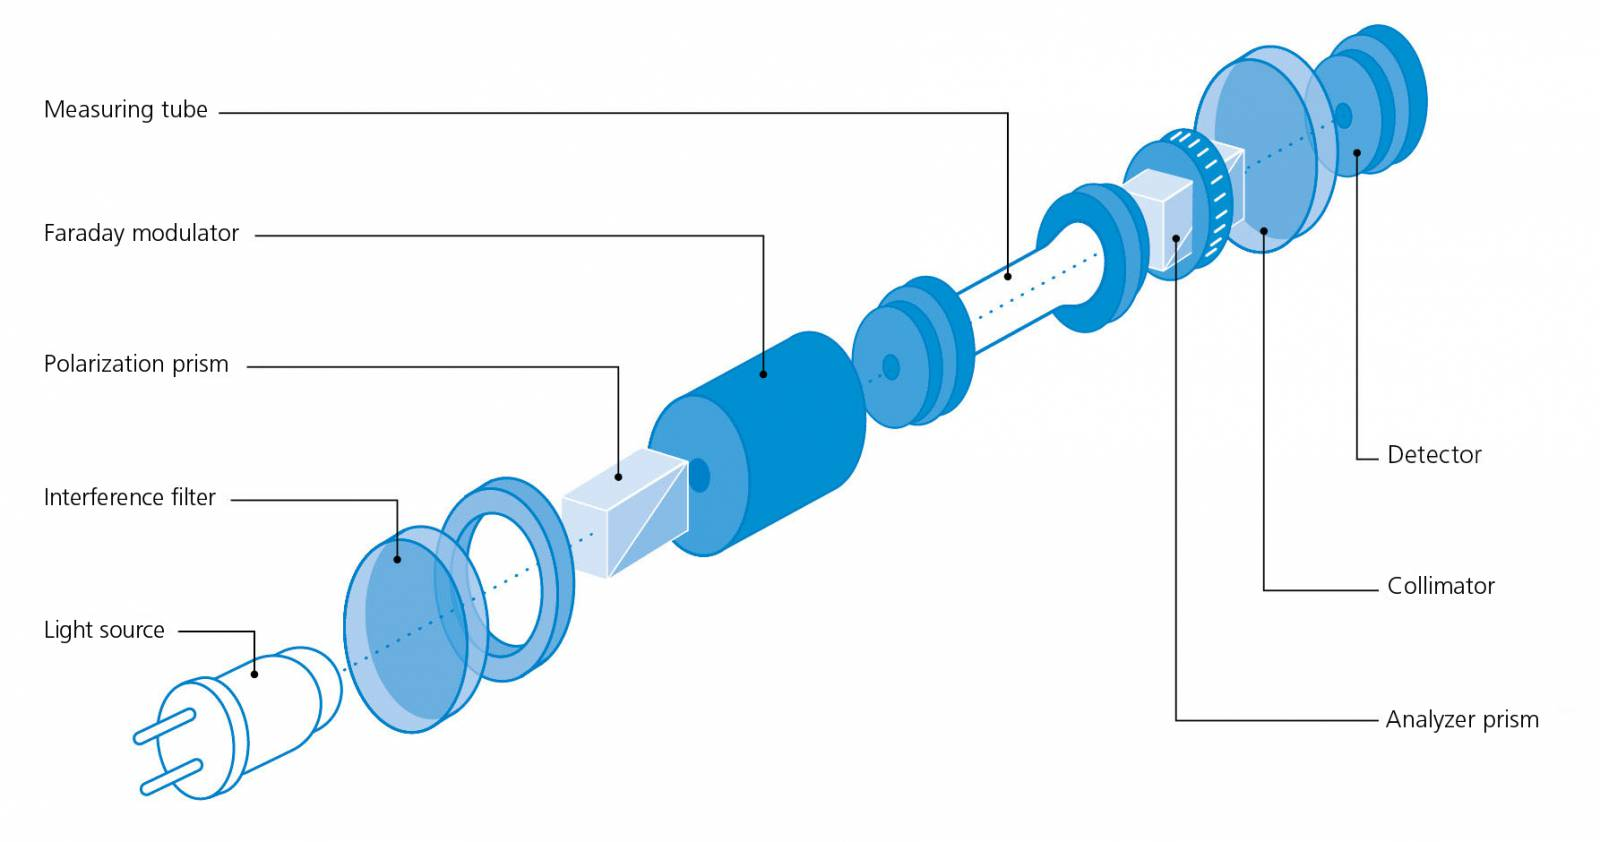
\includegraphics[clip,scale=1,trim={0 0 0 0}]{fig/fig1.jpg}
    \caption{Principle of goniometry}
    \label{figure.9}
        \end{figure} 
      
	\section{Experimental principles}   
	\subsection{Principle of goniometry}
	Measuring the angle between the rays of light is in fact the determination of the azimuth of a parallel beam. A and B are the converging image points of parallel beams 1 and 2 in the focal plane of the telescope. Each point on the focal plane corresponds to a parallel beam incident in a certain direction in a certain direction. If the telescope's optical axis is rotated around the axis of rotation perpendicular to beams 1 and 2, the optical axis is shifted from a direction parallel to beam 1 (the converging image point on the optical axis is A) to the focal plane of the telescope. A) to an orientation parallel to beam 2 (the converging image point on the optical axis is B), the angle through which the optical axis is turned is the angle between parallel beams 1 and 2. The angle of rotation of the optical axis is the angle $\theta $ between beams 1 and 2.
	\begin{figure}[H]
	                  			   					\centering
	                  			   					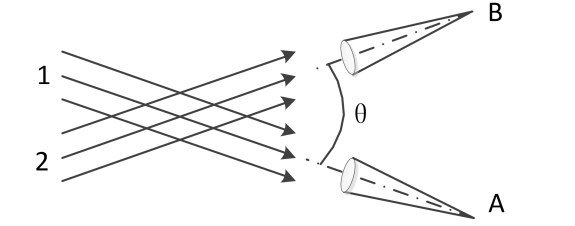
\includegraphics[clip,scale=1,trim={0 0 0 0}]{fig/fig9.png}
	                  			   					\caption{Principle of goniometry}
	                  			   					\label{figure.9}
	                  			   \end{figure} 
     
     \subsection{Half adjustment method}
     Adjust the telescope tilt adjustment screw so that the bright "ten" rises (or falls) by $\frac{h}{2}$, and adjust the carrier Adjust the lower screw b (or c) to raise (or lower) the bright "ten" by $\frac{h}{2}$, as shown in the figure.
     \begin{figure}[H]
         	\centering
         	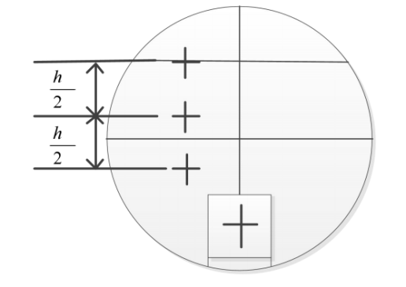
\includegraphics[clip,scale=1,trim={0 0 0 0}]{fig/fig11.png}
         	\caption{Half adjustment method}
         	\label{figure.11}
         	\end{figure} 
     
     
	\subsection{Refractive index measurement by the minimum deflection angle method }
    A beam of monochromatic light is incident on the AB side of a prism at an angle of $\alpha _{1} $, refracted twice by the prism, and then refracted from the AC side at an angle of $\alpha^{’} _{2} $ The angle between the incident light and the outgoing light is called the angle of deflection. The angle $\delta $ between the incident light and the outgoing light is called the angle of deflection. When the top angle A of the prism is fixed, the magnitude of the deflection angle $\delta $ varies with the angle of incidence angle $\alpha _{1} $f. It can be shown that $\delta $ is minimised when $\alpha _{1} = \alpha^{’} _{2}  $ by means of a quotient calculation. The angle of deflection at this point is called the minimum angle of deflection and It is denoted as $\delta_{min} $.
    	\begin{figure}[h]
    	\centering
    	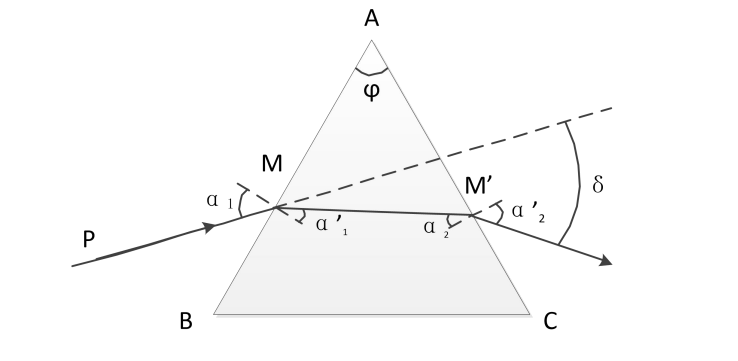
\includegraphics[clip,scale=0.8,trim={0 0 0 0}]{fig/fig10.png}
    	\caption{Refractive index measurement by the minimum deflection angle method}
    	\label{figure.10}
    	\end{figure} 
    	
    Based on the above derivation we can obtain the following equation:
    \begin{eqnarray}
     \alpha ^{'}_1 = \frac{\varphi }{2} 
    \end{eqnarray}
    \begin{eqnarray}
         \delta _{min} = 2\left ( \alpha _1 - \alpha ^{'}_1\right ) = 2\alpha _1 - \varphi  
    \end{eqnarray}     
    \begin{eqnarray}     
         \alpha _1 = \frac{1}{2}\left ( 2\delta _{min} + \varphi   \right )  
    \end{eqnarray}
    
    Let the refractive index of the prism be $n$. Then we have:
    
    \begin{eqnarray}
    \sin \alpha _1 = n\sin \alpha ^{'}_1 = n\sin \frac{\varphi }{2}  
    \end{eqnarray}
    
    Therefore, taking the formula into account we can obtain the following formula for the refractive index:
    \begin{eqnarray}
    n = \frac{\sin \alpha _1}{\sin \frac{\varphi }{2} } = \frac{\sin \frac{1}{2}\left ( \delta _{min} +\varphi \right )  }{\sin \frac{\varphi }{2} } 
    \end{eqnarray}
    
    The top angle $\varphi$ of the prism is given by the laboratory, and the refractive index of the prism material can be calculated experimentally by measuring the minimum deflection angle $\delta _{min}$ from Eq. $n$.
    
	\section{Contents and Steps}
	\subsection{Adjusting spectrometers}
     Before adjusting the spectrophotometer, familiarise yourself with the position of the spectrophotometer's adjustment screws and locking screws and their role.
    \subsubsection{Visual coarse adjustment.} 
    A visual coarse adjustment is an adjustment made by direct observation with the eye. First of all, stand in front of the spectrometer with your eyes in a roughly horizontal position with the telescope, the parallel light tube and the carrier table of the spectrometer. Observe whether the telescope, the parallel light tube and the carrier table are level, and adjust the corresponding screws if they are not: screw 13 for telescope tilt, screw 9 for parallel light tube tilt and screw 3 for carrier table tilt.
    
    If the telescope is not level, adjust the corresponding screws: screw 13 for telescope tilt, screw 9 for parallel light tube tilt and screw 12 for stage tilt as shown in Fig. 3.1-1. The coarse adjustment is the basis and prerequisite for the fine adjustment and must be repeatedly and carefully adjusted to the best possible condition. It makes fine adjustments twice as effective.
    
    \subsubsection{Requirements and steps for fine tuning}
     \begin{itemize}
                 \item Adjust the eyepiece and see clearly the "Feng" forked filament line on the divider. Turn on the power to the small bulb, turn on the switch and observe the lower half of the field of view The green light area in the lower half of the field of view. If so, slowly adjust the eyepiece focus knob until you can clearly see the "fung" forked filament line on the divider and the green "fung" in the green zone.If so, slowly adjust the focus knob of the eyepiece until you can clearly see the green "ten" in the green light area. This is shown in the diagram below:
    \end{itemize}
     \begin{figure}[H]
         	\centering
         	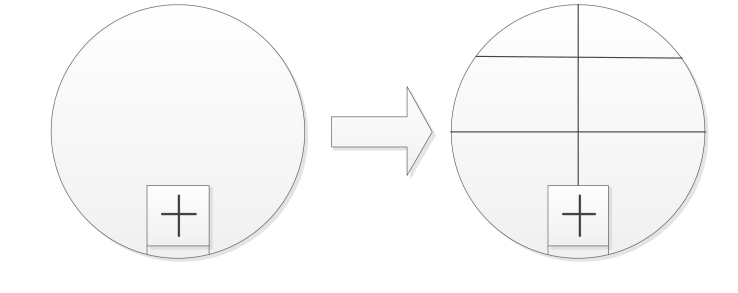
\includegraphics[clip,scale=0.8,trim={0 0 0 0}]{fig/fig12.png}
         	\caption{Field of view change when adjusting the eyepiece}
         	\label{figure.12}
         	\end{figure} 
    \begin{itemize}
                     \item \textbf{Adjust the telescope to suit the reception of parallel light using the self-alignment method:} \\
                     Adjust the carrier stage with three lines dividing the stage in three equal parts, with an angle of 120 degrees between each of the two lines. Place the plane mirror so that it coincides with line a and is perpendicular to the lines b and c . Loosen the carrier screw and adjust the height of the carrier so that the centre of the mirror is at the same height as the telescope axis. Then tighten the screw of the carrier. Loosen the vernier plate locking screw 10, turn the vernier plate (together with the carrier) so that the reflecting mirror is facing the telescope, adjust the telescope tilt adjustment screw or the lower carrier screw b or c as appropriate so that a faint bright spot (or an indistinct bright cross) can be observed in the telescope, loosen the eyepiece sleeve locking screw and move the eyepiece sleeve back and forth until a bright spot is visible. Move the eyepiece sleeve backwards and forwards until a clear bright "ten" is visible and there is no parallax with the sliding plate, at which point the telescope is adjusted to receive parallel light and the sleeve screw is locked in place.
        \end{itemize} 
     \begin{figure}[H]
                          			\begin{minipage}[t]{0.3\linewidth}
                          				\centering
                          				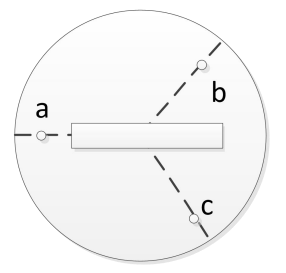
\includegraphics[clip,scale=1.0,trim={0 0 0 0}]{fig/fig13.png}
                          				\caption{ reflector}
                          				\label{figure.13}
                          			\end{minipage}
                          			\begin{minipage}[t]{0.7\linewidth}
                          				\centering
                          				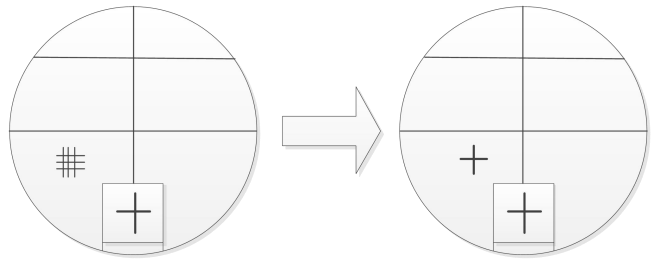
\includegraphics[clip,scale=1,trim={0 4 0 0}]{fig/fig14.png}
                          				\caption{Changes in the field of view when focusing a telescope}
                          				\label{figure.14}
                          			\end{minipage}
                          		\end{figure}

\begin{itemize}
                     \item \textbf{Adjust the optical axis of the telescope perpendicular to the main axis of the spectrometer:} \\
                     the plane reflector is adjusted to the side where the bright "ten" can be seen clearly, and the bright "ten" is modulated by the half-adjustment method to the upper intersection of the forked filaments of the dividing plate. The half adjustment method means that the telescope tilt adjustment screw is adjusted so that the bright ten rises (or falls) by h/2, and the lower screw b (or c) is adjusted so that the bright ten rises (or falls) by h/2.\\
                     After adjusting the bright "ten" to appear in the upper cross position of the dividing plate fork wire, turn the vernier disk (together with the carrier) 180 degrees so that the other side of the reflector is aligned with the telescope, and if the reflected bright "ten" can still be seen in the field of view of the telescope, then Continue to adjust as above, bringing the bright "ten" to the upper intersection of the forked filaments of the dividing plate, and so on several times on both sides of the plane reflector.
                     The telescope's optical axis is perpendicular to the main axis of rotation of the spectrometer.\\
                     If the bright ten reflected from one side of the reflector appears at the upper intersection of the divider, but after 180 degrees of rotation the bright ten reflected from the other side of the reflector is not visible in the telescope (as is often the case during spectrometer adjustment), then Turn the plane mirror back to the side where the bright cross is visible, rather than adjusting blindly on the side where the bright cross is not visible. The correct way to do this is to place the adjusted side against the telescope and adjust the telescope tilt screw so that the bright ten moves down to just below the intersection of the fork wires on the divider, then adjust the screw b (or c) under the carrier so that the bright ten returns to the intersection of the fork wires on the divider. Adjust the screw b (or c) under the carrier to bring the bright cross back to the intersection of the fork wires of the divider. Turn the vernier dial 180 degrees and look in the telescope for the cross.\\
                     If there is a bright ten reflected from the other side of the plane reflector in the telescope, adjust the bright ten to the point of intersection on the fork of the divider according to the half adjustment method; if not, repeat the above adjustments. It is important to note that if the light is not adjusted in the same direction after two consecutive two consecutive adjustments in the same direction, you should consider whether it is time to adjust in a different direction. The adjustment should be made in a different direction.
        \end{itemize} 
     \begin{figure}[H]
                          			\begin{minipage}[t]{0.5\linewidth}
                          				\centering
                          				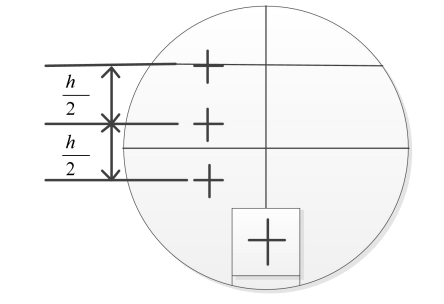
\includegraphics[clip,scale=1.0,trim={0 0 0 0}]{fig/fig15.png}
                          				\caption{ Diagram of each half adjustment}
                          				\label{figure.15}
                          			\end{minipage}
                          			\begin{minipage}[t]{0.5\linewidth}
                          				\centering
                          				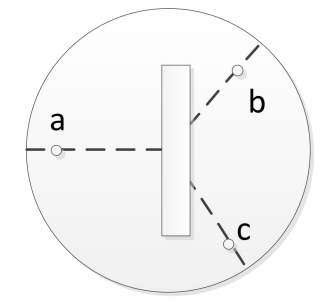
\includegraphics[clip,scale=1,trim={0 0 0 0}]{fig/fig16.png}
                          				\caption{Adjustment of the carrier normal to the rotating spindle}
                          				\label{figure.16}
                          			\end{minipage}
                          		\end{figure}        
 \begin{itemize}
                     \item \textbf{Adjust the carrier normal parallel to the main axis of rotation of the spectrometer:}\\
                     The main purpose of this step is to make the plane swept by the axis of the telescope parallel to the plane of the stage so that the optical elements to be measured (e.g. trigonometric prisms) are placed on the stage with their normal parallel to the optical axis of the telescope.\\
                     On the basis of the adjustments made in step (3) (the telescope tilt screw and the adjustment screws b and c of the stage must not be moved at this point), the flat mirror is removed from the stage.\\
                     The plane mirror is then placed back on the stage so that it is perpendicular to the line a and parallel to the lines b and c. Turn the cursor plate so that the plane reflector is facing the telescope and look for the bright ten reflected back in the field of view, if no bright ten is seen or if the bright ten is not seen If you do not see a bright "ten" or if you see a bright "ten" that does not appear at the intersection of the forked filaments of the divider, adjust only the screw of the carrier a so that the reflected bright ten appears at the upper intersection of the fork filaments of the divider.
                     \item \textbf{Adjust the parallel light tube so that it emits parallel light and make the parallel light tube co-axial with the telescope:}\\
                     Turn on the mercury lamp as the light source, place the slit of the parallel light tube facing the light source, turn the telescope to align the slit of the parallel light tube, loosen the locking screw at the slit, and observe the slit image with the telescope while Adjust the position of the slit sleeve while observing the slit image with the telescope until a clear image of the slit is observed in the telescope (note: the telescope cannot be refocused), and lock the screw on the slit sleeve after the parallel light tube has emitted parallel light. If the slit image is thicker in the telescope, adjust the width of the slit, which is generally best when the width of the slit image is close to the width of the thin line of the forked wire on the slit plate. Adjust the parallel tube tilt adjustment screw so that the slit image is equally divided by the horizontal fork filament in the centre of the dividing plate; adjust the parallel tube coaxial adjustment screw and the telescope coaxial adjustment screw so that the slit image in the field of view of the telescope coincides with the vertical collinear of the dividing plate.
        \end{itemize} 


    
    \subsection{Measuring minimum deflection angles}
   Before measuring, it is important to know the location and function of some common screws. These include the locking screws that control the rotation of the vernier dial; The locking screw that controls the rotation of the telescope and dial together; the locking screw that controls the rotation of the telescope and the screw that controls the micro movement of the telescope.
   \begin{figure}[H]
            	\centering
            	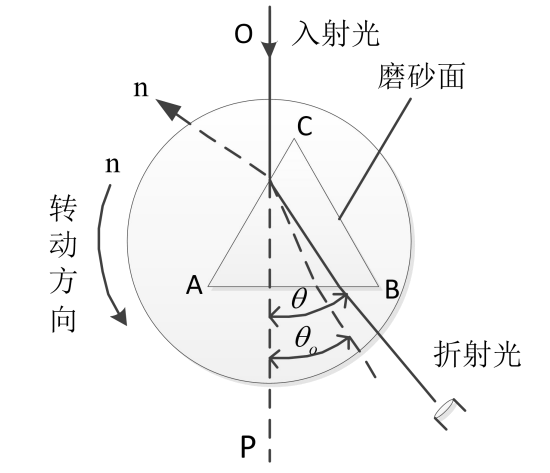
\includegraphics[clip,scale=0.8,trim={0 0 0 0}]{fig/fig17.png}
            	\caption{Measuring minimum deflection angles}
            	\label{figure.17}
            	\end{figure}
   
   \begin{itemize}
       \item The prism has three faces, two of which are smooth and one is ground. When placing the prism, ensure that the light enters from the smooth face and exits from another smooth face.
       \item Loosen the locking screw of the telescope and rotate it in the direction towards the ground face (face BC in the figure) to find the refracted light (slit image) of the prism. At this time, the prism is stationary.
       \item Note that when placing the prism, do not make the ground face BC too vertical to avoid turning the telescope onto the ground face when rotating the eyepiece, which may result in inability to observe.
       \item After finding the refracted bright fringe, select one and keep the eyepiece in the middle. Then gently turn the dial in the opposite direction of rotation until the bright fringe just turns, and the angle of refraction $\alpha _1,\alpha _2$ can be obtained.
       \item Remove the prism, keep the dial still, move the eyepiece back to the initial position P, and record the angles of incidence $\alpha ^{'} _1,\alpha ^{'} _2$.
       \item The minimum deviation angle can be obtained by calculation based on the formula.
       \item The refractive index can be obtained by calculation based on the formula.
   \end{itemize}
   
    The minimum deflection angle is calculated as:
    \begin{eqnarray}
    \theta _{0} = \frac{\left | \alpha _1-\alpha _2 \right | +\left | \alpha ^{'} _1-\alpha ^{'} _2 \right | }{2} 
    \end{eqnarray}
    
    
    
	
	\section{Data processing}
	The experiments were carried out as described above and the following data were subsequently obtained. An error analysis was done on the data and the corresponding results were obtained:
	\subsection{Minimum deflection angle data analysis}
	First we obtained the measured values of the angle $\varphi $ of the top angle of the trigonometric prism and its margin of error based on the following measurements:
   
    \begin{eqnarray}
    \varphi = 60^{\circ} 0^{'} \pm 5^{'} 
    \end{eqnarray}
   
   Subsequently, we followed the experimental steps described above for each of the six experiments. The number of degrees of the wheel to the left and right of the refracted and incident light was measured and recorded, and the minimum angle of deflection was calculated as follows:
   
\begin{table}[htbp]
  \centering
  \caption{Data measurement log sheet}
    \begin{tabular}{cccccc}
    \toprule[2pt]
    \multicolumn{1}{c}{\multirow{2}[0]{*}{Measurement indicators}} & \multicolumn{2}{c}{Refracted light position reading} & \multicolumn{2}{c}{Incident light position reading} &
     \multicolumn{1}{c}{\multirow{2}[0]{*}{$\theta _{0} $}} \\
     \cmidrule{2-3} 
     \cmidrule{4-5}
          & $\alpha_1 $ & $\alpha^{'}_1 $ & $\alpha_2 $ & $\alpha^{'}_2 $ &  \\
    \midrule
    1st   & $33^{\circ}32'$ & $346^{\circ}21'$ & $213^{\circ}35'$ & $166^{\circ}22'$ & $47^{\circ}12'$ \\
    2nd   & $38^{\circ}15'$ & $350^{\circ}55'$ & $218^{\circ}17'$ & $170^{\circ}52'$ & $47^{\circ}18'$ \\
    3rd   & $25^{\circ}08'$ & $337^{\circ}52'$ & $205^{\circ}08'$ & $157^{\circ}50'$ & $47^{\circ}17'$ \\
    4th   & $295^{\circ}56'$ & $342^{\circ}48'$ & $115^{\circ}54'$ & $162^{\circ}48'$ & $46^{\circ}52'$ \\
    5th   & $300^{\circ}35'$ & $347^{\circ}45'$ & $210^{\circ}36'$ & $257^{\circ}47'$ & $47^{\circ}10'$ \\
    6th   & $28^{\circ}33'$ & $75^{\circ}49'$ & $208^{\circ}35'$ & $255^{\circ}53'$ & $47^{\circ}17'$ \\
    \bottomrule[2pt]
    \end{tabular}%
  \label{tab:addlabel}%
\end{table}%

   To improve the accuracy of the experimental data, we analysed the anomalies in the $\theta _0$ values before calculating the refractive index. First we calculate their mean and standard deviation as follows:
   \begin{eqnarray}
   \bar{\theta _0}  = \frac{\sum_{i=1}^{6}\theta _{0_{i} }  }{6} =47^{\circ} 11'
   \end{eqnarray}
   \begin{eqnarray}
   \sigma _{\theta _{0} } =\sqrt{\frac{ {\textstyle \sum_{i=1}^{6}}\left ( \bar{\theta _{0_i}} - \theta _{0_i}\right )^2  }{6}   } = 9' 
   \end{eqnarray}
   
    Based on the data at this point we can conclude that the measured value of $\theta _0$ is:
    \begin{eqnarray}
    \theta _0 = 47^{\circ} 11'\pm 9'
    \end{eqnarray}
    
    For the information in the table, we tried to remove outliers. Two methods were used to identify outliers: one was to analyse the data for outliers by plotting a standard box plot, and the other was to calculate the mean and standard deviation, treating data that were more or less than double the standard deviation of the mean as outliers (marked as red dots in the graph). Box line plots and scatter plots based on the above approaches are as follows:
     \begin{figure}[H]
                              			\begin{minipage}[t]{0.5\linewidth}
                              				\centering
                              				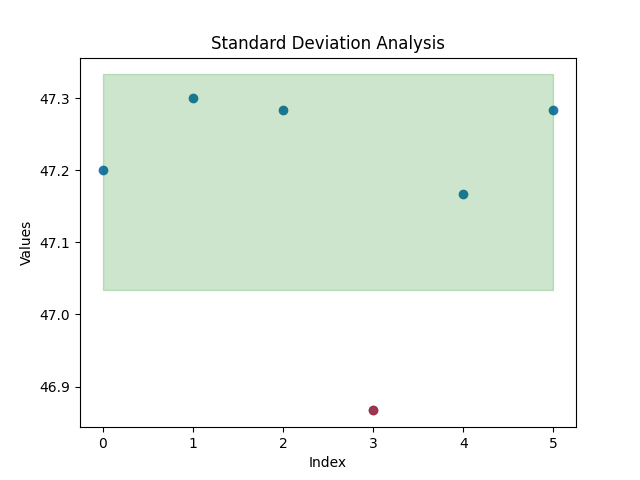
\includegraphics[clip,scale=0.5,trim={0 0 0 0}]{fig/fig18.png}
                              				\caption{ Scatter plot outlier analysis}
                              				\label{figure.18}
                              			\end{minipage}
                              			\begin{minipage}[t]{0.5\linewidth}
                              				\centering
                              				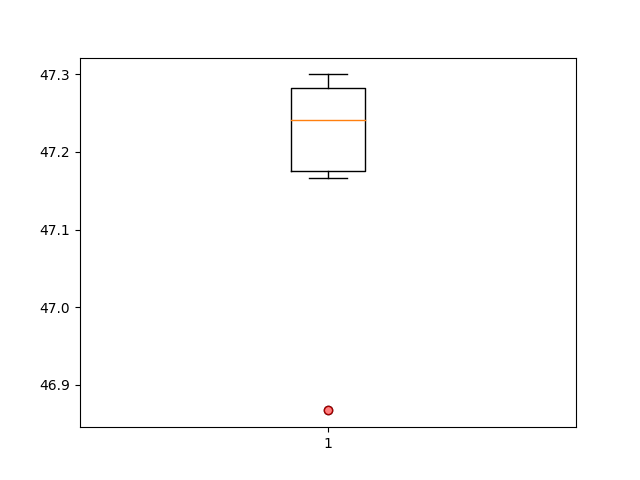
\includegraphics[clip,scale=0.5,trim={0 0 0 
                              				0}]{fig/fig19.png}
                              				\caption{Box line chart outlier analysis}
                              				\label{figure.19}
                              			\end{minipage}
                              		\end{figure} 
     
    As we can see from the graphs, when analysed using both the box line and scatter plots are, we can find only one clear outlier in the data: the data from the fourth experiment. Therefore, we chose to ignore the data from that experiment. The new data was obtained as follows, and we also took the new data into the equation to calculate the final refractive index which is also recorded in the table below.
    
    \begin{table}[htbp]
      \centering
      \caption{Data measurement log sheet}
        \begin{tabular}{ccccccc}
        \toprule[2pt]
        \multicolumn{1}{c}{\multirow{2}[0]{*}{Measurement indicators}} & \multicolumn{2}{c}{Refracted light position reading} & \multicolumn{2}{c}{Incident light position reading} &
         \multicolumn{1}{c}{\multirow{2}[0]{*}{$\theta _{0} $}} & \multicolumn{1}{c}{\multirow{2}[0]{*}{$n$}} \\
         \cmidrule{2-3} 
         \cmidrule{4-5}
              & $\alpha_1 $ & $\alpha^{'}_1 $ & $\alpha_2 $ & $\alpha^{'}_2 $ &  \\
        \midrule
        1st   & $33^{\circ}32'$ & $346^{\circ}21'$ & $213^{\circ}35'$ & $166^{\circ}22'$ & $47^{\circ}12'$ & 1.610\\
        2nd   & $38^{\circ}15'$ & $350^{\circ}55'$ & $218^{\circ}17'$ & $170^{\circ}52'$ & $47^{\circ}18'$ & 1.611\\
        3rd   & $25^{\circ}08'$ & $337^{\circ}52'$ & $205^{\circ}08'$ & $157^{\circ}50'$ & $47^{\circ}17'$ & 1.611\\
        5th   & $300^{\circ}35'$ & $347^{\circ}45'$ & $210^{\circ}36'$ & $257^{\circ}47'$ & $47^{\circ}10'$ & 1.610\\
        6th   & $28^{\circ}33'$ & $75^{\circ}49'$ & $208^{\circ}35'$ & $255^{\circ}53'$ & $47^{\circ}17'$ & 1.611\\
        \bottomrule[2pt]
        \end{tabular}%
      \label{tab:addlabel}%
    \end{table}%
    

    \subsubsection{Refractive index numerical analysis}
   After completing the refractive index calculations, we obtained a total of five sets of refractive index data without anomalies. We re-analysed these five sets of data in the same way as we had previously analysed the anomalies to obtain the following results:
   \begin{eqnarray}
   \bar{n}  = \frac{\sum_{i=1}^{5}n_i  }{5} =1.6106
   \end{eqnarray}
   \begin{eqnarray}
    \sigma _{n } =\sqrt{\frac{ {\textstyle \sum_{i=1}^{5}}\left ( \bar{n} - n_i\right )^2  }{5}   } = 0.0005 
   \end{eqnarray}
   
  Thus, we find the final refractive index result to be:
  \begin{eqnarray}
  n = 1.6106\pm 0.0005
  \end{eqnarray}
   
   
   
  
\section{Conclusion and analysis}
\subsection{Experimental conclusion}

Based on the information from the data obtained from the experiments and the results of the data processing, we can obtain the final resluts:

\begin{align*}
  n = 1.6106\pm 0.0005
\end{align*}

This experiment used a spectrophotometer to measure the refractive index of the trigonal prism, and the equipment as well as the experimental procedure actually interfered less with the results. The results are therefore first correct and more accurate.

However, the experiment may be subject to some error, which we will focus on in the next section

\subsection{Experimental error analysis}
\begin{itemize}
\item Reading error: Due to the limited human visual ability, it may not be possible to accurately read the scale on the vernier plate, or there may be visual fatigue or other factors that cause reading deviation.
\item Instrument error: Each component in the spectrometer may have a certain degree of error, such as the parallelism between the parallel light tube and the parallel plane mirror, the perpendicularity between the prism and the base, etc.
\item Environmental factors: Temperature, humidity, air pressure, vibration, and other environmental factors may also affect the accuracy of the experiment.
\item Human factors: The operation of the experimenter may also affect the accuracy of the experiment, such as the stability of hand holding the vernier knob, the degree of alignment between the light source and the prism, etc.
\end{itemize}

It is necessary to carefully control these possible errors during the experiment to ensure the accuracy of the measurement results.

\begin{appendix}
	\section{Data Analysis and Visualisation Source Code}
	\subsection{Calculation of data means and standard deviations}
	\begin{lstlisting}[language=python]
import numpy as np
import matplotlib.pyplot as plt
# 定义数据
#data = np.array([47.2,	47.3,	47.283,	46.867,	47.167,	47.283])
data = np.array([1.61,	1.611,	1.611,	1.61,	1.611])
mean = np.mean(data)
std = np.std(data)
print(mean,std)
	\end{lstlisting}
	
	\subsection{Box line charting and outlier analysis}
	\begin{lstlisting}[language=python]
import numpy as np
import matplotlib.pyplot as plt

# 读取数据
#data = np.array([47.2,	47.3,	47.283,	46.867,	47.167,	47.283])
data = np.array([1.61,	1.611,	1.611,	1.61,	1.611])

# 绘制箱线图
fig, ax = plt.subplots()
ax.boxplot(data)

# 标记异常值
q1 = np.percentile(data, 25)
q3 = np.percentile(data, 75)
iqr = q3 - q1
upper_bound = q3 + 1.5 * iqr
lower_bound = q1 - 1.5 * iqr
outliers = [x for x in data if x < lower_bound or x > upper_bound]
ax.plot(np.ones(len(outliers)), outliers, 'ro', alpha=0.5)

# 显示图形
plt.show()
		\end{lstlisting}
		
	\subsection{Scatter plot production and outlier analysis}
		\begin{lstlisting}[language=python]
import numpy as np
import matplotlib.pyplot as plt

# 读取数据
#data = np.array([47.2,	47.3,	47.283,	46.867,	47.167,	47.283])
data = np.array([1.61,	1.611,	1.611,	1.61,	1.611])

# 计算平均值和标准差
mean = np.mean(data)
std = np.std(data)

# 计算异常值阈值
threshold = mean +  std
down = mean -  std
# 绘制散点图
fig, ax = plt.subplots()
ax.scatter(range(len(data)), data)

# 标记异常值
outliers = [x for x in data if x > threshold or x<down]
ax.plot([i for i in range(len(data)) if data[i] in outliers], outliers, 'ro', alpha=0.5)

# 添加阴影
x = np.linspace(0, len(data)-1, 100)
y1 = mean - std
y2 = mean + std
ax.fill_between(x, y1, y2, alpha=0.2, color='green')

# 设置图形属性
ax.set_title('Standard Deviation Analysis')
ax.set_xlabel('Index')
ax.set_ylabel('Values')

# 显示图形
plt.show()

		\end{lstlisting}

\end{appendix}


\end{document}  